%=============================================================================
%  IEEE-format report (8 pages target)
%  Compile with pdflatex (twice).  Figures are read from signed_bench/.
%=============================================================================
\documentclass[journal,letterpaper,10pt]{IEEEtran}

\usepackage{amsmath,amssymb}
\usepackage{graphicx}
\usepackage{booktabs}
\usepackage{multirow}
\usepackage{array}
\usepackage{listings}
\usepackage{xcolor}
\usepackage{url}
\usepackage{balance}

\lstdefinestyle{pycode}{
  language=Python,
  basicstyle=\ttfamily\scriptsize,
  keywordstyle=\bfseries,
  commentstyle=\itshape\color{gray},
  numbers=left,
  numberstyle=\tiny\color{gray},
  numbersep=4pt,
  frame=single,
  rulecolor=\color{gray!60},
  framesep=2pt,
  breaklines=true,
  breakatwhitespace=false,
  breakindent=10pt,
  postbreak=\mbox{\textcolor{gray}{$\hookrightarrow$}\space},
  columns=fullflexible,
  keepspaces=true,
  showstringspaces=false,
  aboveskip=4pt,
  belowskip=4pt,
  captionpos=b
}

\begin{document}

\title{Optimised Artificial Bee Colony Search for Influence Maximisation on Signed Trust Networks}

\author{Tanubhav~Juneja and Tarundeep~Singh% TODO: replace with the final author block
\thanks{Manuscript prepared November 2026. Code, data and per-cell result files accompany this report.}}

\maketitle

\begin{abstract}
Influence maximisation on signed trust networks is usually studied with models borrowed from the independent-cascade literature, where an active seed either converts a neighbour or does not. Trust networks behave differently: a person who has taken a side pulls neighbours toward that side, and a negative edge carries the opposite opinion. This report evaluates an optimised Artificial Bee Colony (ABC) searcher under a two-opinion signed majority rule on three public networks: Bitcoin Alpha (3{,}783 nodes), Bitcoin OTC (5{,}881) and Slashdot (82{,}140). It is compared with canonical ABC, the ABCVNS algorithm of Tang \emph{et al.} (both the published LIE fitness and a majority-rule surrogate), signed PageRank and weighted degree. Across 117 measured cells, the optimised ABC returns the highest net spread on Bitcoin Alpha at $k=10$ and $k=20$, beats canonical ABC on eight of nine graph--budget pairs, and is 27--41\,\% faster than the fixed ABCVNS variant on Slashdot (mean 35\,\%). The study also shows that maximising positive spread is not the same as maximising net spread: the ABCVNS surrogate gains 154--248 negative activations on Bitcoin OTC and loses 12--14\,\% of net spread for it. Diversity and community fairness are reported alongside spread, and a calibration procedure puts every wall-clock measurement on one GPU basis.
\end{abstract}

\begin{IEEEkeywords}
Influence maximisation, signed networks, majority rule, artificial bee colony, ABCVNS, opinion dynamics.
\end{IEEEkeywords}

%=============================================================================
\section{Objective}
%=============================================================================

A signed trust network records both who trusts whom and who distrusts whom. Picking $k$ accounts to seed is the influence-maximisation problem on such a graph, but the optimisation is only half of it; the diffusion rule decides what the numbers mean. On Bitcoin Alpha a positive rating means one user trusted another with money, and a negative rating means a reported scam. Slashdot's Zoo network is the same idea in a discussion community: friend and foe tags, no money involved. Seeding a set of users and watching opinions propagate is the natural question a moderator would ask, and it is not answered by models that treat activation as a one-way infection. Signed influence maximisation has been studied with friend/foe cascades \cite{li2013}, and threshold models of collective behaviour go back to Granovetter \cite{granovetter1978}; what the two literatures rarely do is put opinions, signs and a fixed evaluation budget in the same experiment.

The standard machinery assumes submodularity. Kempe, Kleinberg and Tardos showed that for independent cascade and linear threshold the expected spread is a monotone submodular function of the seed set, which is what makes the greedy $(1-1/e)$ guarantee work \cite{kempe2003} and what lets CELF skip most re-evaluations \cite{leskovec2007}; the sufficient condition behind the result is submodularity of the local activation function \cite{mossel2007}. Under a majority rule with signed influence neither property survives in the form the algorithms need. The function remains monotone---more seeds never hurt---but the marginal gain of a node can rise after another node is added. The smallest witness, found first on the unsigned model, is a three-leaf star: adding the second leaf can be worth three activations where the first was worth one. Our audit of the lazy bound in the validation suite found 418 violations in 832 re-checks (50.2\,\%), and the set CELF picked differed from exact greedy in 16 of 17 graph--budget configurations, scoring strictly lower in 13 of them. CELF is still a useful warm start. It is not a guarantee.

ABCVNS, the algorithm in the paper this project started from \cite{tang2026}, brings a strong search layer: an elite-global cooperative neighbourhood, three variable-neighbourhood-search tiers, and population management. Its fitness, however, is a closed-form independent-cascade surrogate (LIE) that never looks at edge signs and rewards dense two-hop rings. On the signed majority rule that objective points the wrong way. Measured on Bitcoin Alpha at $k=10$, the published variant placed its seeds in neighbourhoods where a single active seed could flip nothing, and the held-out spread came out at 10.2---barely above the seed count---against 595.2 for the same search machinery with a majority-aware surrogate. The search was fine; the objective was not.

The model has a history in this project that is worth stating plainly. It was first studied on unsigned graphs---Watts--Strogatz, Barab\'asi--Albert and stochastic block models---where monotonicity was proved, the non-submodularity witnesses were machine-checked, and the nine ABC operators were tuned. Extending it to signed graphs took two steps: edge signs enter the support sum, and nodes gain opinions. The operators were designed for the unsigned plateau, so whether they survive the signed extension is an empirical question, and it is the one this benchmark answers.

This work has four objectives. The first is to define a signed majority rule that actually represents opinions: nodes end positive-active, negative-active or inactive, and a negative edge flips the opinion it carries rather than merely subtracting weight. The second is to measure how far an optimised ABC---whole-$k$-set search with nine operator repairs---gets under that rule at a fixed evaluation budget. The third is a controlled comparison against canonical ABC, ABCVNS in its published and repaired forms, signed PageRank and weighted degree on three public networks, scoring positive, negative and net spread together with opinion diversity, community fairness and wall-clock time. The fourth is methodological: to put every timing on a single hardware basis, because the benchmark straddled a period when the GPU backend was unavailable and a mixed table would have misranked the algorithms.

The scope is deliberately bounded. Budgets are $k\in\{10,20,30\}$, the three graphs are used as published, and the comparison is at equal evaluation budget rather than equal wall-clock. Temporal graphs, $k=100$, memory profiling and the independent-cascade regime are outside this report; the cascade results for ABCVNS's home model are reported separately in the project's real-network study. No claim of optimality is made anywhere. The claims are comparisons between implemented algorithms under one protocol.

%=============================================================================
\section{Our Approach}
%=============================================================================

\subsection{Two-Opinion Signed Majority Rule}

Each node $v$ holds a state $s_v\in\{-1,0,+1\}$: negative-active, inactive, positive-active. Every node draws a threshold $\theta_v\sim U[0.35,0.65]$ once per Monte-Carlo draw, and $\deg(v)$ is the total absolute weight incident to $v$. An active neighbour $u$ contributes
\begin{equation}
c_{u\to v} \;=\; \operatorname{sign}(e_{uv})\, s_u\, w_{uv},
\label{eq:contrib}
\end{equation}
so a positive edge passes $u$'s opinion through and a negative edge delivers its opposite. The net support is
\begin{equation}
S_v \;=\; \sum_{u\in N(v)} c_{u\to v},
\label{eq:support}
\end{equation}
and an inactive node joins with the sign of its support when the support clears its personal threshold:
\begin{equation}
s_v \leftarrow \operatorname{sign}(S_v)
\quad\text{if}\quad |S_v| > \theta_v \deg(v).
\label{eq:activate}
\end{equation}
The process is progressive; an active node never changes side. Seeds are planted at $+1$, since the question is which users to recruit, and negative-active nodes arise only through the dynamics. A node whose support is exactly zero stays inactive: there is no tie-breaking rule, because a tie is not a majority.

An earlier implementation in this project treated nodes as binary active/inactive and assigned polarity afterwards from the sign of their incident edges. That formulation cannot represent a node being pulled to the opposite side by a negative edge, and it makes the negative spread a property of the graph rather than of the cascade. All results in this report use \eqref{eq:contrib}--\eqref{eq:activate}. Two consequences matter for the search. Adding a seed can lower the net spread, because a badly placed positive seed can flip a region negative: on Bitcoin Alpha, adding one pool node to a $k=10$ set raised positive spread from 551.9 to 576.4 and negative spread from 10.5 to 38.8, so net spread fell from 541.4 to 537.7. And the gain landscape has plateaus: many seed sets produce identical cascades, so a searcher that only compares final spread has no gradient to follow.

\subsection{Searching Whole $k$-Sets}

The search variable is a set $S$ of $k$ distinct nodes drawn from a candidate pool of 200. Its objective is the expected number of positive-active nodes at convergence,
\begin{equation}
\sigma^{+}(S) \;=\; \mathbb{E}\bigl[\#\{v : s_v=+1\}\bigr],
\label{eq:sigma}
\end{equation}
estimated by Monte Carlo over $R_{\mathrm{fit}}=30$ frozen threshold vectors. Because $\sigma^{+}$ is flat across large regions, the fitness adds a plateau potential computed in the same cascade pass,
\begin{equation}
\Phi(S)=\sum_{v\ \text{inactive}} \min\!\left(1,\frac{\max(S_v,0)}{\theta_v\deg(v)}\right),
\label{eq:phi}
\end{equation}
and ranks candidates by $\sigma^{+}+\lambda\Phi$ with $\lambda=0.05$. Comparisons between two candidates are made lexicographically on $(\sigma^{+},\Phi)$, with a tolerance of twice the standard error of the Monte-Carlo mean, so that noise does not masquerade as improvement.

The budget is $k\times 200$ fresh cascade evaluations per restart, the exact cost of running greedy over the pool, and every solver is held to it. The colony has 30 food sources (15 employed bees) and runs at most 80 cycles. Initialisation is a CELF warm start plus degree-biased random sets; because the best-ever set is retained, a restart can never finish below its own CELF seed. The CELF implementation counts lazy-bound violations rather than assuming them away.

\begin{lstlisting}[style=pycode,caption={Audited CELF lazy bound. Violations are counted, not suppressed.},label={lst:celf}]
while len(S) < k and heap:
    neg_g, v, last_round = heapq.heappop(heap)
    if last_round == len(S):            # bound computed on the current set
        S.append(v); cur += -neg_g; continue
    new_g = model.sigma(S + [v]) - cur  # stale bound: re-evaluate
    checks += 1
    if new_g > stale[v] + 1e-9:
        violations += 1                 # submodularity violated
    stale[v] = new_g
    heapq.heappush(heap, (-new_g, v, len(S)))
\end{lstlisting}

\subsection{Nine Operator Repairs}

Canonical ABC was designed for continuous functions \cite{karaboga2005,karaboga2007}, and its discrete translation has failure modes that show up immediately on set-valued search. Each repair below targets one of them; the parameters are the ones used in every reported run.

\begin{enumerate}
\item \emph{Weak exploitation.} With probability $0.6$ a bee takes the global-best set as its partner instead of a random colony member \cite{zhu2010}, so late moves copy from the incumbent rather than from noise.
\item \emph{Roulette collapse.} Onlookers are chosen by tournament of size 4, not by fitness-proportional sampling; near-identical fitness values then still produce a ranking.
\item \emph{Blind scouts.} An abandoned source is rebuilt near the incumbent in 70\,\% of cases (two forced swaps, every slot re-rolled) and fully at random in the remaining 30\,\% \cite{kiran2015}.
\item \emph{Fixed perturbation.} Each candidate receives one partner-guided swap plus, with probability $0.2$, one extra random swap \cite{akay2012}. Step size and diversity are controlled separately.
\item \emph{Duplicate sources.} Exact duplicate sets are replaced by fresh biased samples, and the replacement count is recorded.
\item \emph{Budget exhaustion by refinement.} 15\,\% of the budget is reserved for local refinement and every refinement call receives only what is left. In the reported runs refinement is disabled (\texttt{refine\_every=0}), so the entire budget goes to the colony.
\item \emph{Rigid moves on plateaus.} $\Phi$ breaks ties, equal-fitness moves are accepted when they improve $\Phi$, and with probability $0.15$ a move is a fresh random set.
\item \emph{Stale refinement.} Two consecutive refinement passes that swap nothing switch refinement off for the rest of the run and return its reserve to the colony.
\item \emph{Coalitions one-swap cannot repair.} When one-swap stalls, up to 400 two-swap attempts are made, with swap-ins restricted to neighbours of the current seeds and of near-threshold nodes.
\end{enumerate}

\begin{lstlisting}[style=pycode,caption={ABC cycle (excerpt): gbest partners, tournament onlookers, directed scouts, dedupe and elitism.},label={lst:abc}]
for cycle in range(1, cfg.max_cycles + 1):
    if not budget_left():
        break
    for i in range(n_sources):                  # employed bees
        partner = (best_set if rng.random() < cfg.gbest_prob
                   else population[rng.integers(n_sources)])
        cand = _candidate(population[i], partner, pool, k, rng, cfg)
        ns, nph, nse = fitness_of(cand)
        if accept(ns, nph, nse, i):
            population[i], fit_pairs[i] = cand, (ns, nph, nse)
            trials[i] = 0
        else:
            trials[i] += 1
    for i in _pick_sources(fitness, rng, cfg):  # onlooker bees
        partner = best_set if rng.random() < cfg.gbest_prob \
                  else population[rng.integers(n_sources)]
        cand = _candidate(population[i], partner, pool, k, rng, cfg)
        if accept(*fitness_of(cand), i):
            population[i] = cand; trials[i] = 0
    for i in range(n_sources):                  # scouts
        if trials[i] > cfg.limit:
            if cfg.directed_scout and rng.random() < 0.7:
                cand = _neighbour_solution(best_set, best_set,
                                           pool, k, rng, cfg)
            else:
                cand = rng.choice(pool, size=k, replace=False).tolist()
            population[i] = cand; trials[i] = 0
    if cfg.dedupe:
        dedupe()
    i = int(np.argmax([s for s, _, _ in fit_pairs]))
    if fit_pairs[i][0] > best_fit:              # elitism
        best_fit, best_set = fit_pairs[i][0], list(population[i])
\end{lstlisting}

\subsection{ABCVNS and Its Majority-Rule Surrogate}

The reference algorithm \cite{tang2026} runs the same kind of set search but scores candidates with LIE, a closed form derived for independent cascade:
\begin{equation}
\mathrm{LIE}(S)=|S|+\Bigl(1+p\,\tfrac{\sum_{u\in N_2}d_u^{*}}{|N_1|}\Bigr)
\sum_{i\in N_1}\bigl(1-(1-p)^{c_i}\bigr),
\label{eq:lie}
\end{equation}
where $N_1$ is the one-hop shell of $S$, $N_2$ the two-hop shell, $c_i$ the number of seeds adjacent to $i$, and $d_u^{*}$ an edge count inside the ring. No Monte-Carlo evaluation is performed during its search. The rest of the machinery is the paper's: elite-global cooperative neighbourhood construction for employed and onlooker bees, tournament onlookers with $t_s=3$, bifurcated scouts, three VNS tiers (score-driven one-swap, betweenness-oriented two-hop swap, community-aware swap with retention $r=0.2$) plus a local search over the top $c_n=10$ score-ranked neighbours, and population management on stagnation. Parameters are $g_{\max}=150$, $NP=50$, $r=0.2$, $c_n=10$, $L=5$, $\tau_{\max}=5$, $m_{\max}=3$, $\alpha=0.5$, with $p=0.05$ on the Bitcoin graphs and $p=0.01$ on Slashdot.

The repaired variant keeps every line of that search and replaces only the scalar. The surrogate propagates \emph{signed} net mass two hops and converts it to an activation probability using the model's own threshold distribution. With $c$ the expected net mass reaching $v$,
\begin{equation}
P_v(c)=\operatorname{clamp}\!\left(\frac{c/\deg(v)-(0.5-\delta)}{2\delta},0,1\right),
\label{eq:prob}
\end{equation}
and
\begin{equation}
\mathrm{Score}(S)=|S|+\sum_{i\in N_1}P_i(c_i)+\sum_{j\in N_2}P_j(c_j'),
\label{eq:mr}
\end{equation}
where $c_j'$ is the mass arriving when the one-hop shell is replaced by its expected activation probability. The signed scatter is the same quantity the diffusion thresholds, so enemy edges pull the score down instead of being ignored.

\begin{lstlisting}[style=pycode,caption={Majority-rule surrogate fitness used by the repaired ABCVNS.},label={lst:mr}]
cnt1 = st.dot_signed(s_dev)                 # signed net mass, one hop
p1 = be.clip((cnt1 / safe - st.lo) / st.width, 0.0, 1.0)
p1[s_dev == 1] = 0.0
n1 = cnt1 != 0
n1[s_dev == 1] = False

e = s_dev + p1                              # expected active mass
score = float(k) + float(p1.sum())

cnt2 = st.dot_signed(e)                     # two-hop net mass
p2 = be.clip((cnt2 / safe - st.lo) / st.width, 0.0, 1.0)
p2[s_dev == 1] = 0.0
p2[n1] = 0.0
return score + float(p2.sum())
\end{lstlisting}

%=============================================================================
\section{Findings and Results}
%=============================================================================

Every number in this section is held out: seed sets were scored on $R_{\mathrm{ho}}=300$ fresh threshold draws that the search never saw, and averaged over restarts. Table~\ref{tab:net} gives the headline metric. Fig.~\ref{fig:net} plots the same values against $k$.

\begin{table*}[!t]
\centering
\caption{Net spread (positive minus negative), held-out, mean $\pm$ standard deviation over restarts.}
\label{tab:net}
\scriptsize
\setlength{\tabcolsep}{3.5pt}
\begin{tabular}{@{}lccccccccc@{}}
\toprule
& \multicolumn{3}{c}{Bitcoin Alpha} & \multicolumn{3}{c}{Bitcoin OTC} & \multicolumn{3}{c}{Slashdot}\\
\cmidrule(lr){2-4}\cmidrule(lr){5-7}\cmidrule(lr){8-10}
Algorithm & $k{=}10$ & $k{=}20$ & $k{=}30$ & $k{=}10$ & $k{=}20$ & $k{=}30$ & $k{=}10$ & $k{=}20$ & $k{=}30$\\
\midrule
ABC (proposed)   & $542.7\pm1.1$  & $769.7\pm2.6$   & $958.0\pm5.0$   & $857.3\pm1.8$  & $1124.2\pm2.4$  & $1319.2\pm2.3$  & $1717.4\pm23.9$ & $2226.8\pm23.5$ & $2529.6\pm5.3$\\
ABC (canonical)  & $539.2\pm3.6$  & $748.3\pm15.5$  & $915.2\pm19.8$  & $855.9\pm3.7$  & $1110.4\pm7.8$  & $1276.2\pm25.5$ & $1725.1\pm17.9$ & $2089.6\pm94.3$ & $2453.8\pm49.0$\\
ABCVNS (fixed)   & $538.5\pm0.8$  & $747.0\pm13.1$  & $953.6\pm7.3$   & $754.7\pm8.0$  & $964.7\pm20.0$  & $1159.4\pm16.7$ & $1770.4\pm56.3$ & $2151.7\pm71.0$ & $2367.6\pm55.0$\\
SignedPageRank   & $538.6$        & $765.2$         & $962.9$         & $860.9$        & $1106.3$        & $1334.4$        & $1811.3$        & $2256.6$        & $2615.6$\\
Degree           & $394.0$        & $653.8$         & $770.8$         & $508.9$        & $726.9$         & $879.0$         & $1700.7$        & $1975.3$        & $2170.8$\\
\bottomrule
\end{tabular}
\end{table*}

\begin{figure*}[!t]
\centering
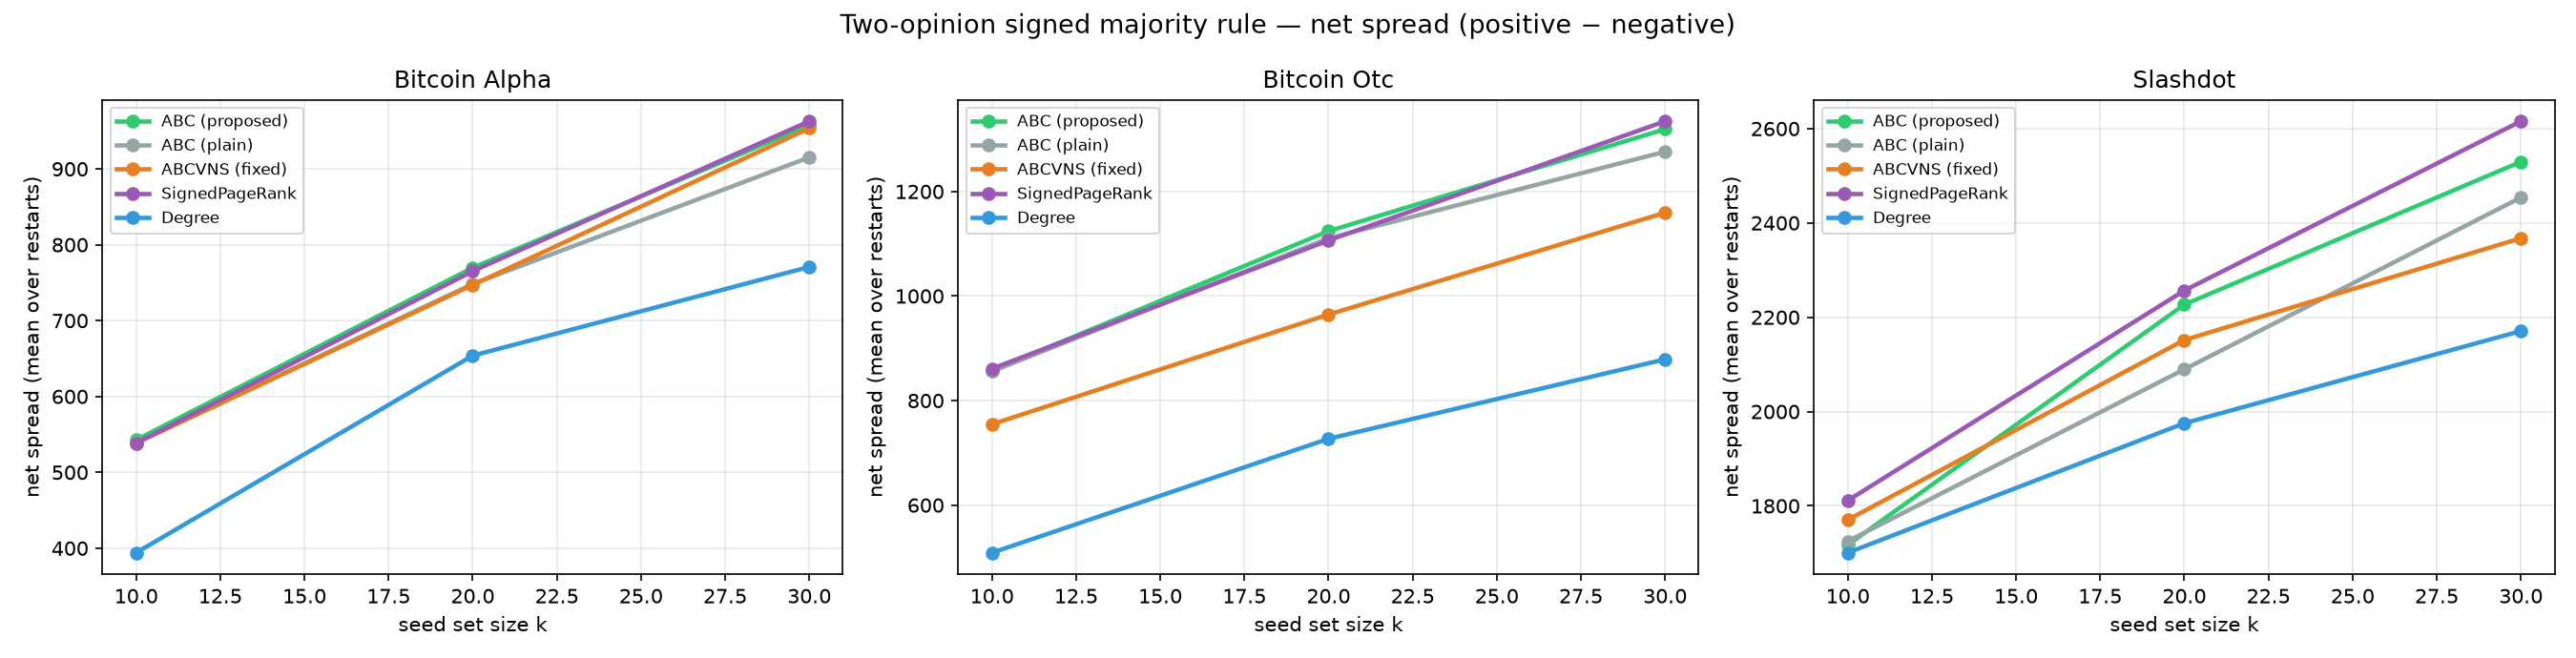
\includegraphics[width=0.92\textwidth]{signed_bench/opinion_spread.png}
\caption{Net spread against seed-set size for the five algorithms. The optimised ABC leads on Bitcoin Alpha at $k=10$ and $k=20$; signed PageRank is the strongest static method on Slashdot.}
\label{fig:net}
\end{figure*}

\subsection{Net Spread}

Bitcoin Alpha separates the field. The optimised ABC returns 542.7, 769.7 and 958.0 positive-minus-negative nodes at $k=10,20,30$. Signed PageRank is within 0.8\,\% at every budget and edges ahead at $k=30$ (962.9 against 958.0), while the repaired ABCVNS is close behind (538.5--953.6). Degree centrality \cite{freeman1978} loses 15--27\,\% of net spread on Alpha and 33--41\,\% on OTC; its seeds are hubs, and hubs sit in neighbourhoods that the majority rule cannot flip.

On Bitcoin OTC the ordering changes. Signed PageRank wins at $k=10$ (860.9 against 857.3) and $k=30$ (1334.4 against 1319.2), and the optimised ABC wins at $k=20$ (1124.2). The gap to the repaired ABCVNS is the largest in the study: 102.6, 159.5 and 159.8 net nodes at the three budgets, or 12--14\,\%. That gap is not a spread failure; it is a sign failure, discussed next.

Slashdot rewards the static ranking. Signed PageRank is best at all three budgets (1811.3, 2256.6, 2615.6), with the optimised ABC second (1717.4, 2226.8, 2529.6) and the repaired ABCVNS third. The absolute numbers are small next to the graph size---2{,}530 net activations on 82{,}140 nodes at $k=30$, about 3\,\%---which is what a 0.35--0.65 threshold does on a sparse graph.

The comparison with canonical ABC is the cleanest signal for the operator set. The optimised version is ahead in eight of nine cells, with gains of 3.5/21.4/42.8 on Alpha, 1.4/13.8/43.0 on OTC, and 137.2/75.8 at $k=20/30$ on Slashdot; the one loss, $-7.7$ at Slashdot $k=10$, sits inside the restart standard deviation (23.9). Restart variance is also lower almost everywhere, which matters for a method that will be run once in practice.

\subsection{Positive and Negative Components}

Splitting the spread exposes what the net figure hides. On OTC the repaired ABCVNS has the highest positive spread at $k=10$ (909.1) and stays within 0.2--1\,\% of the best at $k=20$ and $k=30$ (1175.7 and 1407.8), yet it also produces 154.4, 211.0 and 248.4 negative-active nodes. The optimised ABC produces 871.4, 1152.0 and 1356.1 positive nodes with only 14.1, 27.8 and 36.9 negative ones. Positive-only objectives pay for their extra reach in opposition.

Degree centrality shows the same pattern more starkly: 709--1192 positive nodes against 200--313 negative ones. On Slashdot the negative component is small for every method (6.4--52.0), so the net and positive rankings coincide there. The lesson is not that negative spread should be minimised to zero---some of it is unavoidable on a signed graph---but that a fitness which ignores it will buy positive activations at a poor exchange rate.

\begin{table*}[!t]
\centering
\caption{Positive spread (upper) and negative spread (lower) at $k=30$, held-out, mean over restarts.}
\label{tab:posneg}
\scriptsize
\setlength{\tabcolsep}{4pt}
\begin{tabular}{@{}lcccccc@{}}
\toprule
& \multicolumn{3}{c}{Positive spread} & \multicolumn{3}{c}{Negative spread}\\
\cmidrule(lr){2-4}\cmidrule(lr){5-7}
Algorithm & Alpha & OTC & Slashdot & Alpha & OTC & Slashdot\\
\midrule
ABC (proposed)   & $1011.9$ & $1356.1$ & $2555.0$ & $54.0$  & $36.9$  & $25.3$\\
ABC (canonical)  & $969.2$  & $1313.2$ & $2479.1$ & $53.9$  & $37.0$  & $25.3$\\
ABCVNS (fixed)   & $1026.5$ & $1407.8$ & $2408.4$ & $72.9$  & $248.4$ & $40.8$\\
SignedPageRank   & $1003.0$ & $1418.4$ & $2631.6$ & $40.2$  & $84.0$  & $16.0$\\
Degree           & $872.2$  & $1191.8$ & $2222.8$ & $101.4$ & $312.9$ & $52.0$\\
\bottomrule
\end{tabular}
\end{table*}

\subsection{Diversity}

Opinion diversity is the normalised binary entropy of the final opinions among active nodes, so 0 means a one-sided cascade and 1 means an even split. Degree centrality is the most diverse method everywhere: 0.43--0.48 on Alpha and 0.74--0.76 on OTC. That is a by-product of reaching many low-threshold regions at once, and it comes with the lowest net spread in the study. The repaired ABCVNS is next on OTC (0.60--0.62), again because its cascades recruit both sides. The optimised ABC is the least diverse on OTC (0.12--0.18) and near the bottom on Alpha (0.12--0.29). Slashdot compresses everyone: 0.03--0.16, with the optimised ABC at 0.04--0.08.

There is a real trade-off here and no free setting. If the goal is a broad, mixed conversation, degree seeding delivers it at a large cost in net reach. If the goal is to move as many nodes as possible to the positive side, the optimised ABC does that while producing a narrow outcome. Reporting both is more honest than choosing one and calling it quality.

\begin{figure*}[!t]
\centering
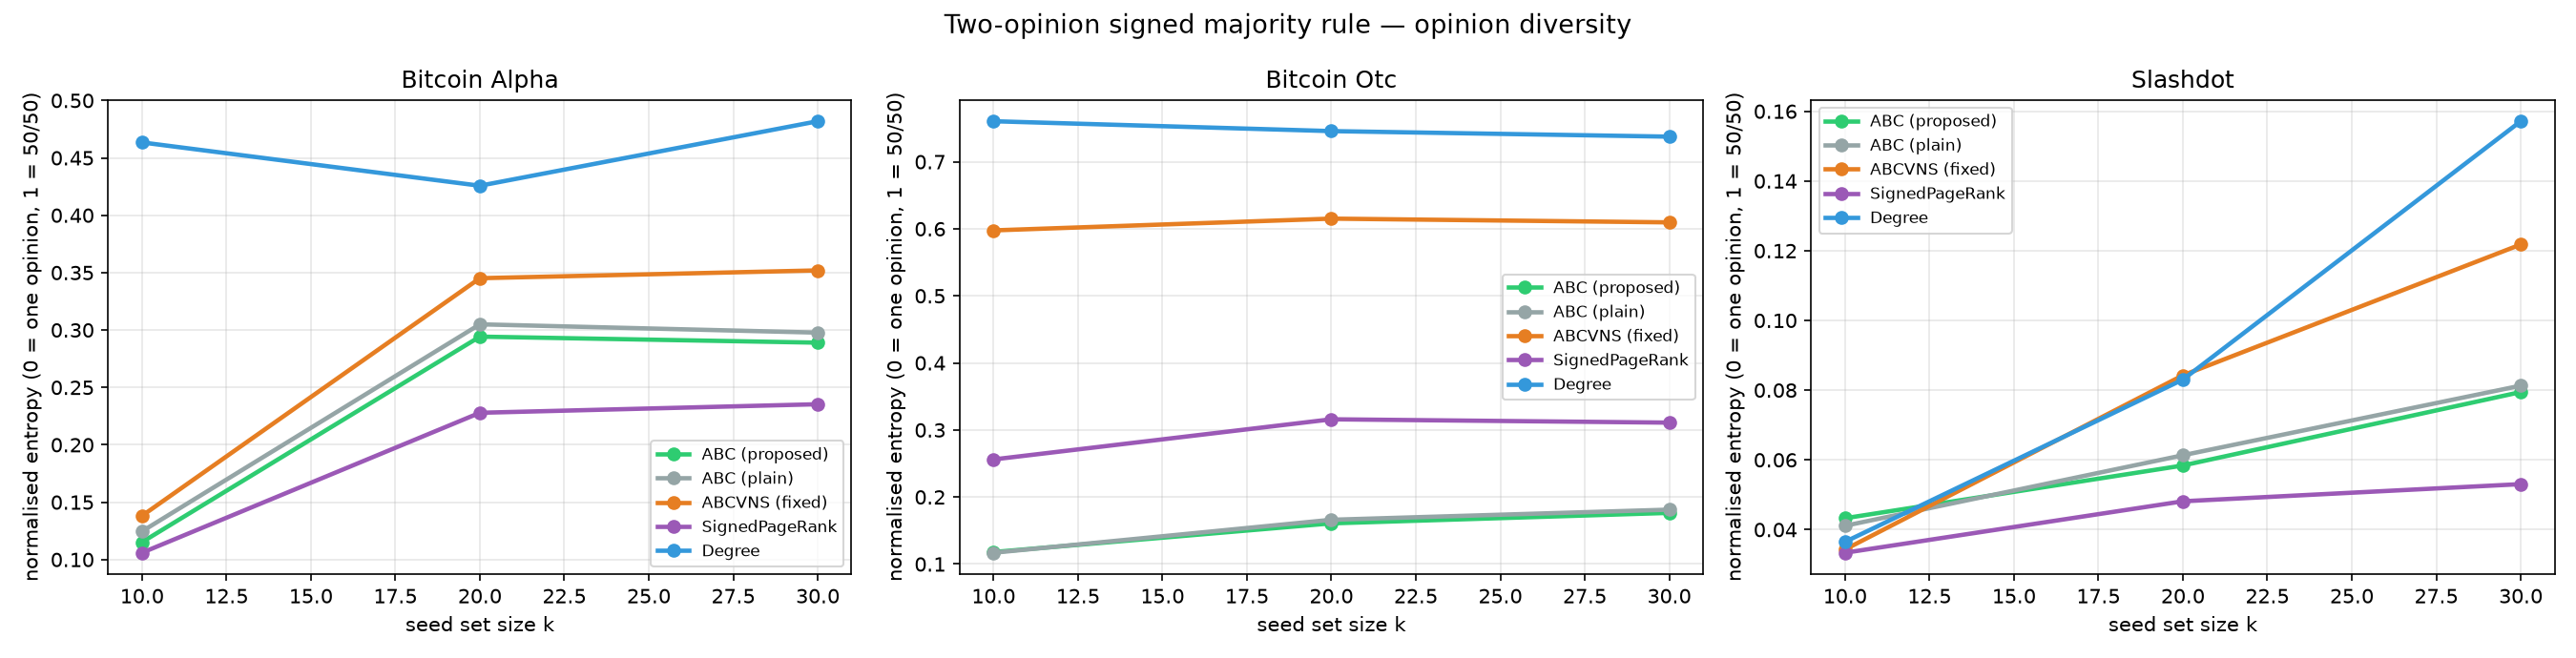
\includegraphics[width=0.92\textwidth]{signed_bench/opinion_diversity.png}
\caption{Opinion diversity (normalised entropy of final opinions among active nodes) against seed-set size. Degree seeding keeps the cascade mixed; the optimised ABC concentrates it.}
\label{fig:div}
\end{figure*}

\subsection{Community Fairness}

Fairness is measured over Louvain communities with at least ten nodes: $F=1-(\max_c a_c-\min_c a_c)$, where $a_c$ is the fraction of community $c$ that ends active. A value of 1 means every community is reached equally; 0 means one community is fully activated while another is untouched. The metric is deliberately harsh, and the numbers should be read that way.

On Slashdot the optimised ABC, canonical ABC and degree seeding all sit at 0.35--0.37, the repaired ABCVNS at 0.12--0.18 with large restart swings (standard deviations up to 0.16), and signed PageRank at 0.01--0.07. On the Bitcoin graphs every method collapses toward zero once $k$ reaches 20: some community saturates, the maximum rate hits 1, and the minimum stays near 0. The optimised ABC is at 0.004--0.006 there, not because it is unfair in any absolute sense but because the metric's range is exhausted. A fairness-constrained objective would need a different functional, for example a size-weighted variance of activation rates; the max-minus-min definition is kept because it is transparent and was fixed before the runs.

\begin{figure*}[!t]
\centering
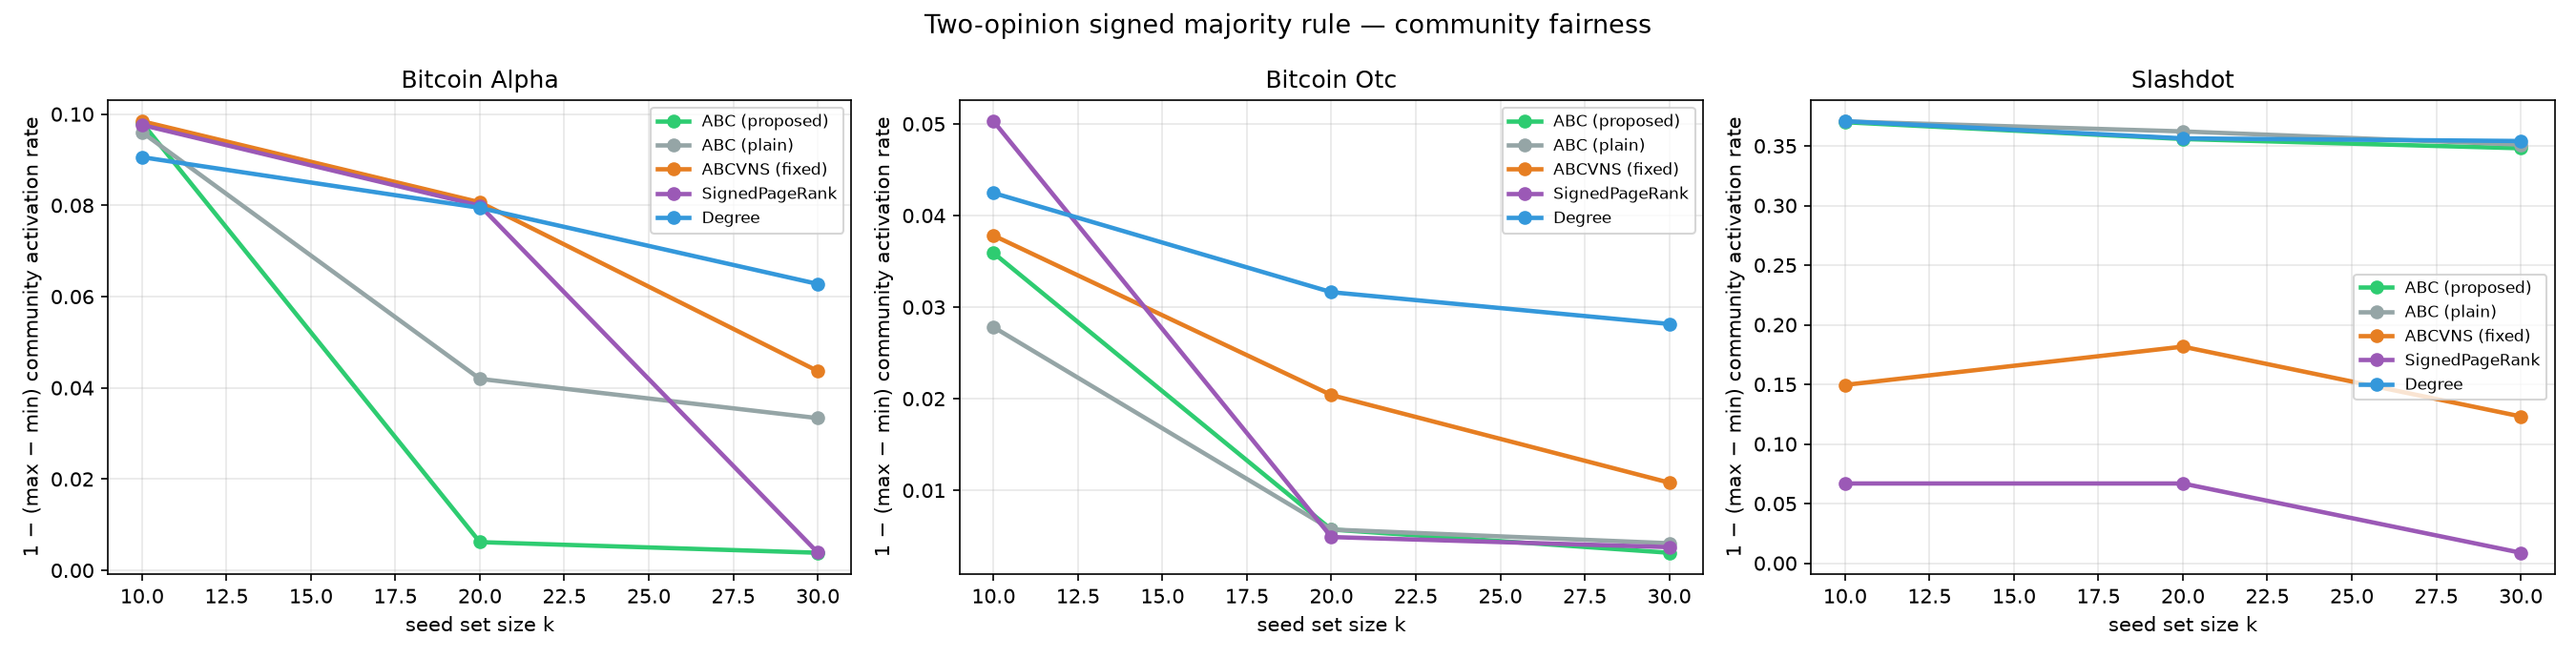
\includegraphics[width=0.92\textwidth]{signed_bench/opinion_fairness.png}
\caption{Community fairness against seed-set size. Slashdot separates the methods; on the Bitcoin graphs the max-minus-min range saturates and every method collapses toward zero.}
\label{fig:fair}
\end{figure*}

\subsection{Wall-Clock}

Table~\ref{tab:time} reports seconds per restart on the common GPU basis described in Section~\ref{sec:timing}. On Slashdot the optimised ABC takes 48.4, 54.1 and 56.7 s against 65.9, 87.9 and 96.4 s for the repaired ABCVNS: 27\,\%, 38\,\% and 41\,\% faster, 35\,\% on average. On Bitcoin the gap is wider in relative terms (58--73\,\%) because ABCVNS performs tens of thousands of small LIE operations whose launch overhead dominates on a 3--6k-node graph. The absolute times there are 12--22 s against 40--68 s.

Canonical ABC is faster than the optimised one on Slashdot (30.3 s against 48.4 s at $k=10$), and the difference is the CELF warm start: about 18 s of the $k=10$ run is spent evaluating the lazy-greedy seed set. The warm start pays for itself in spread at $k=20$ and $k=30$ and in the guarantee that a restart cannot fall below CELF, but it is a real cost at small $k$ and should be reported as one. Both baselines are effectively free (0.02--0.04 s), which is the honest reason signed PageRank remains attractive on Slashdot despite losing on Bitcoin Alpha.

\begin{table*}[!t]
\centering
\caption{Wall-clock seconds per restart on the common GPU basis, mean $\pm$ standard deviation over restarts.}
\label{tab:time}
\scriptsize
\setlength{\tabcolsep}{3.5pt}
\begin{tabular}{@{}lccccccccc@{}}
\toprule
& \multicolumn{3}{c}{Bitcoin Alpha} & \multicolumn{3}{c}{Bitcoin OTC} & \multicolumn{3}{c}{Slashdot}\\
\cmidrule(lr){2-4}\cmidrule(lr){5-7}\cmidrule(lr){8-10}
Algorithm & $k{=}10$ & $k{=}20$ & $k{=}30$ & $k{=}10$ & $k{=}20$ & $k{=}30$ & $k{=}10$ & $k{=}20$ & $k{=}30$\\
\midrule
ABC (proposed)   & $11.9\pm0.3$ & $20.1\pm0.4$ & $22.4\pm0.7$ & $12.2\pm0.4$ & $17.4\pm0.1$ & $18.5\pm0.3$ & $48.4\pm0.1$ & $54.1\pm0.3$ & $56.7\pm0.3$\\
ABC (canonical)  & $11.9\pm0.3$ & $18.3\pm0.6$ & $20.7\pm0.5$ & $11.8\pm0.3$ & $15.8\pm0.4$ & $17.6\pm0.2$ & $30.3\pm0.3$ & $35.3\pm0.8$ & $37.1\pm0.9$\\
ABCVNS (fixed)   & $39.6\pm1.7$ & $48.0\pm1.9$ & $60.6\pm3.3$ & $39.7\pm0.7$ & $43.0\pm1.4$ & $68.2\pm3.7$ & $65.9\pm0.9$ & $87.9\pm2.3$ & $96.4\pm3.2$\\
SignedPageRank   & $0.02$ & $0.02$ & $0.02$ & $0.02$ & $0.02$ & $0.02$ & $0.02$ & $0.02$ & $0.02$\\
Degree           & $0.04$ & $0.04$ & $0.04$ & $0.04$ & $0.04$ & $0.04$ & $0.04$ & $0.04$ & $0.04$\\
\bottomrule
\end{tabular}
\end{table*}

\subsection{Restart Stability}

The standard deviations in Table~\ref{tab:net} carry information the means hide. The optimised ABC is the most stable searcher on Bitcoin, with standard deviations of 0.4--5.0 spread units on Alpha and 0.2--2.4 on OTC across three restarts. The repaired ABCVNS ranges from 0.8 on Alpha to 71.0 on Slashdot, and canonical ABC reaches 94.3 on Slashdot. On Slashdot the optimised ABC varies by 5.3--23.9 units at spreads above 1{,}700, under 1.4\,\%. The repaired ABCVNS is the least stable method there (standard deviations 55--71), which is consistent with its VNS tiers landing in different basins depending on the initial population. A method whose restarts disagree by 3--4\,\% needs more restarts before its mean can be trusted; a method whose restarts agree within 1\,\% can be run once.

\subsection{Relation to the Published ABCVNS Timings}

The ABCVNS paper reports its Slashdot run at $k=100$ as $1.08\times10^{4}$\,s (about three hours) against $6.48\times10^{5}$\,s (about 7.5 days) for CELF with a 1{,}000-draw Monte-Carlo oracle \cite{tang2026}. Our numbers cannot be compared to those directly, and it is worth saying why. The budget here is $k\le30$, the oracle is 30 GPU draws rather than 1{,}000 CPU draws, and CELF is not part of the corrected benchmark. What the comparison does show is where ABCVNS's cost sits: its search performs tens of thousands of LIE evaluations and no Monte-Carlo draws, so on a GPU it is bound by kernel-launch overhead on small graphs (39.6--68.2\,s on Bitcoin, where the optimised ABC needs 11.9--22.4\,s) and by the sheer evaluation count on Slashdot (65.9--96.4\,s). The paper's speed advantage over CELF is a statement about lazy greedy with an expensive oracle. It is not evidence that the ABCVNS search itself is cheap.

\subsection{What the Numbers Say}

Three claims survive the full table and nothing stronger does: the optimised ABC is the strongest searcher on Alpha, a positive-only surrogate loses net spread exactly where signs are dense, and static sign-aware ranking is hard to beat on Slashdot at a cost four orders of magnitude smaller. Everything else in the table is a trade-off between those poles.

%=============================================================================
\section{Test Procedure}
%=============================================================================

\subsection{Networks}

The three graphs are the public SNAP releases used in the signed-network literature \cite{kumar2016,kunegis2009,kunegis2010,leskovec2010}. Multi-ratings between the same pair are collapsed to one edge keeping the largest absolute weight, self-loops are dropped, and directed edges are treated as undirected, following the project convention. Table~\ref{tab:data} lists the sizes. The Slashdot release is the February 2009 Zoo network; the ABCVNS paper used a different Slashdot snapshot (70{,}069 nodes), so absolute spreads are not directly comparable to its figures, although the algorithm behaviour is.

\begin{table}[!t]
\centering
\caption{Networks after collapsing multi-edges and symmetrising.}
\label{tab:data}
\footnotesize
\setlength{\tabcolsep}{3pt}
\begin{tabular}{@{}lrrrr@{}}
\toprule
Network & Nodes & Edges & Positive & Negative\\
\midrule
Bitcoin Alpha & 3{,}783 & 14{,}124 & 12{,}806 & 1{,}318\\
Bitcoin OTC   & 5{,}881 & 21{,}492 & 18{,}333 & 3{,}159\\
Slashdot      & 82{,}140 & 500{,}481 & 382{,}167 & 118{,}314\\
\bottomrule
\end{tabular}
\end{table}

\subsection{Diffusion Engine and Scoring}

The cascade is evaluated for all $R$ threshold draws at once. Each round scatters the frontier's signed influence into a per-node, per-draw support matrix, then activates every inactive node whose support clears its threshold, taking the sign of the support as the new opinion. On the CPU path the scatter uses \texttt{np.add.at} over flat indices; on the GPU path the same operation is a single \texttt{index\_put\_} with accumulation. Edge chunks of 40{,}000 keep peak memory inside 6\,GB of VRAM on the 82k-node graph.

\begin{lstlisting}[style=pycode,caption={One diffusion round over all $R$ draws (CPU path; the GPU path is the same operation with a scatter kernel).},label={lst:diff}]
while frontier.any():
    e = frontier[src].any(axis=1)           # edges leaving the frontier
    s_sel, d_sel, w_sel = src[e], dst[e], sw[e]
    fr = frontier[s_sel].astype(np.float32)
    idx = d_sel[:, None] * R + rr[None, :]  # (edges, draws) flat indices
    np.add.at(support.ravel(), idx.ravel(),
              (w_sel[:, None] * fr).ravel())
    newly = (np.abs(support) >= need) & (active == 0)
    sgn = (support > 0).astype(np.int8) - (support < 0).astype(np.int8)
    active = np.where(newly, sgn, active)   # opinion = sign of support
    frontier = newly
\end{lstlisting}

Weights are integers on all three graphs (ratings of 1--10 on Bitcoin, $\pm1$ on Slashdot), so the support sums are exact in single precision and the CPU and GPU paths produce identical cascades. That was checked directly: the same seed sets scored on both backends returned the same positive, negative and net counts to the last node, which is why converting timings between backends does not change any spread value. Each evaluation costs $O(mR)$ in the worst case, since every round touches each edge once per draw; a restart of the optimised ABC therefore costs $O(k\cdot200\cdot mR)$, and a restart of ABCVNS costs $O(E_{\mathrm{LIE}}\,m)$ with $E_{\mathrm{LIE}}$ in the tens of thousands.

Search draws use a fixed threshold tensor (seed 7); held-out scoring uses a separate tensor (seed 999{,}999). Every algorithm sees the same draws within a stage, and final seed sets are scored only on the held-out tensor.

\subsection{Protocol}

Budgets are $k\in\{10,20,30\}$; the candidate pool is 200 nodes for every graph, built from four rankings---net positive support, PageRank \cite{page1999}, $k$-core and low-threshold nodes---plus a random tail of 25\,\%. Each restart gets $k\times200$ fresh cascade evaluations, the exact cost of running greedy over the pool. The cap is enforced by a counter checked before every bee move, and it includes the warm-start evaluations, so a restart cannot exceed the cap even when the colony is still improving. Restart counts are 3 for the optimised ABC, 3 for canonical ABC, 5 for the repaired ABCVNS and 1 for the two deterministic baselines, which do not benefit from restarts. Search-time estimation uses $R_{\mathrm{fit}}=30$ draws; held-out scoring uses $R_{\mathrm{ho}}=300$. Random states are fixed per restart (\texttt{random\_state=600+rs} for ABC), so a cell can be reproduced exactly.

The repaired ABCVNS uses the paper's IC probability in its LIE context ($p=0.05$ on Bitcoin, $p=0.01$ on Slashdot) even though the diffusion is the majority rule; the surrogate itself uses $\delta=0.15$, matching the model. This keeps the comparison to the published algorithm's configuration and isolates the fitness change.

\begin{table}[!t]
\centering
\caption{Configurations used in every reported run.}
\label{tab:params}
\footnotesize
\setlength{\tabcolsep}{3pt}
\begin{tabular}{@{}ll@{}}
\toprule
\multicolumn{2}{@{}l}{\emph{ABC (proposed); canonical values in brackets}}\\
Colony size / cycles & 30 / 80\\
gbest partner probability & 0.6 (0.0)\\
Onlooker selection & tournament, size 4 (roulette)\\
Abandonment limit & 6\\
Partner swaps / mutation rate & 1 / 0.2\\
Random exploration probability & 0.15 (0.0)\\
Plateau weight $\lambda$ & 0.05 (0.0)\\
Acceptance tolerance & $2\times$ standard error\\
Budget & $k\times200$ evaluations\\
Restarts & 3\\
\midrule
\multicolumn{2}{@{}l}{\emph{ABCVNS (published and fixed)}}\\
Generations / population & 150 / 50\\
Tournament size & 3\\
Retention ratio $r$ & 0.2\\
Local-search width $c_n$ & 10\\
Stagnation $L$ / $\tau_{\max}$ / $m_{\max}$ & 5 / 5 / 3\\
Score blend $\alpha$ & 0.5\\
IC probability $p$ & 0.05; 0.01 on Slashdot\\
Restarts & 5\\
\bottomrule
\end{tabular}
\end{table}

\subsection{Metrics}

Positive spread is the mean number of nodes ending at $+1$; negative spread the mean at $-1$; net spread is their difference. All three are held-out means over restarts. Diversity is the normalised binary entropy
\begin{equation}
H=\frac{-p_+\log_2 p_+ - p_-\log_2 p_-}{\log_2 2},
\label{eq:div}
\end{equation}
with $p_\pm$ the share of each opinion among active nodes, and $H=0$ when one side is empty. Fairness is
\begin{equation}
F=1-\bigl(\max_{c} a_c-\min_{c} a_c\bigr),\qquad a_c=\frac{|A\cap C_c|}{|C_c|},
\label{eq:fair}
\end{equation}
over Louvain communities \cite{blondel2008} with $|C_c|\ge10$; communities smaller than ten nodes were excluded because a single activation in a five-node community produces a rate of 0.2 that says nothing about reach.

\subsection{Putting Timings on One Basis}
\label{sec:timing}

The benchmark ran across a period when Windows Smart App Control began blocking the unsigned PyTorch DLLs, which forced the Bitcoin cells and the first Slashdot $k=10$ cells onto the numpy CPU path. The raw table was therefore incomparable: Slashdot $k=10$ showed 419.7 s for the optimised ABC and $k=20$ showed 54.1 s for the same algorithm, a drop caused entirely by the backend switch.

Rather than discard the completed cells, we measured the conversion on the same machine. Microbenchmarks gave the per-evaluation ratio for the two workloads: on Slashdot a diffusion evaluation cost 108.3 ms on CPU and 9.4 ms on GPU (11.5$\times$), and an LIE evaluation 9.78 ms against 0.92 ms (10.6$\times$). On small graphs the GPU is slower for LIE (0.183 ms CPU against 0.739 ms GPU on Alpha) because the operation is dominated by kernel-launch overhead. Six GPU anchor runs of the exact configurations then fixed the end-to-end ratios: Slashdot ABC at $k=10$ 420.8 s $\to$ 48.5 s (8.68$\times$); Alpha ABC 13.0 s $\to$ 12.2 s; Alpha ABCVNS 9.5 s $\to$ 39.8 s; OTC ABC 23.6 s $\to$ 12.6 s; OTC ABCVNS 11.1 s $\to$ 39.4 s. The ABCVNS Slashdot ratio (8.60$\times$) came from its own dual-backend cells.

Converted rows are marked \texttt{estimated\_gpu} in the result CSV; measured rows are \texttt{measured\_gpu}; the two structural baselines are \texttt{structural}. The original measurement is preserved in a \texttt{time\_raw\_s} column next to every converted value, so any claim in this report can be traced back to the raw number. Spreads needed no conversion: as noted above, the two backends agree exactly.

\subsection{Reproducibility}

Every finished cell is appended to \texttt{results\_opinion.csv} immediately and skipped on re-run, which is how the benchmark survived a mid-run backend switch and a machine restart without recomputing a single cell. The runner logs one line per cell with graph, $k$, algorithm, restart, wall-clock and all five spread metrics.

\begin{lstlisting}[style=pycode,caption={Resumable cell loop: finished work is never recomputed.},label={lst:runner}]
done = load_done()
for k in ks:
    for alg in algs:
        for rs in range(restarts[alg]):
            key = (name, k, alg, rs)
            if key in done:
                continue
            row = one_cell(name, G, k, alg, rs, model, ho,
                           metrics, pool, st_mr)
            append_cell(row)
            done.add(key)
\end{lstlisting}

Hardware: an Intel i9-14900HX laptop CPU with 32\,GB of RAM, an NVIDIA RTX 3060 Laptop GPU with 6\,GB, driver 591.44 (CUDA 13.1), PyTorch 2.14.1+cu126, Python 3.15 on Windows 11. The code is plain numpy plus an optional torch backend; no networkx or scipy is used in the benchmark path.

%=============================================================================
\section{Conclusion and Future Scope}
%=============================================================================

The corrected model changes the answer. Under a two-opinion signed majority rule, the optimised ABC is the strongest searcher on Bitcoin Alpha at every budget (542.7, 769.7, 958.0 net nodes) and beats canonical ABC on eight of nine graph--budget pairs. On Bitcoin OTC it wins at $k=20$ and trails signed PageRank by 0.4--1.1\,\% at the other two budgets. On Slashdot it is second to signed PageRank at every budget but 27--41\,\% faster than the repaired ABCVNS, and the speed advantage is stable across budgets (mean 35\,\%).

The most useful negative result is about objectives. Maximising positive spread alone does not maximise net spread: the repaired ABCVNS buys 154--248 negative activations on OTC and gives up 12--14\,\% of net spread for them. Any signed-network searcher that scores only one side of the cascade is optimising a proxy, and the proxy is expensive exactly where the signs are dense.

Diversity and fairness behave as constraints rather than objectives. Degree seeding produces the most mixed opinions on the Bitcoin graphs and matches the best community coverage on Slashdot, at a 15--27\,\% loss of net spread on Alpha. The optimised ABC does the opposite. Reporting both makes the trade-off visible; a single composite score would hide it.

Future work falls into four lines. The first is a multi-objective fitness, $\sigma^{+}-\beta\,\sigma^{-}$ with $\beta$ calibrated per graph, which the OTC result suggests is the right shape. The second is a learned surrogate: fit the two-hop activation model from Monte-Carlo traces so that a cheap fitness tracks the actual diffusion instead of a fixed closed form. The third is engineering: batch the VNS candidate evaluations into single GPU kernels, parallelise restarts, and extend the benchmark to $k=100$ on Slashdot, where the paper's own CELF run takes days. The fourth is theoretical: a submodular envelope for the signed majority rule, in the spirit of the sandwich bounds used for other non-submodular diffusions, would turn the current heuristics into algorithms with guarantees.

Three limitations should be stated plainly. Restart counts are 3 and 5, not the paper's 30, because 30 restarts on Slashdot would take days of wall-clock; the standard deviations in Table~\ref{tab:net} show that the ordering is stable, but a formal significance test would need more restarts. The operator set is justified by the ABC-versus-canonical-ABC comparison, not by a fresh leave-one-out ablation under the signed model: the operators were tuned on the unsigned problem, and re-running the ablation is future work. And the timing conversion, while anchored on real GPU runs of the same configurations, is an estimate for the converted cells; the measured and estimated rows are labelled so that a reader can restrict attention to the measured ones.

\begin{thebibliography}{17}

\bibitem{kempe2003}
D. Kempe, J. Kleinberg, and \'E. Tardos, ``Maximizing the spread of influence through a social network,'' in \emph{Proc. 9th ACM SIGKDD Int. Conf. Knowledge Discovery and Data Mining}, 2003, pp. 137--146.

\bibitem{leskovec2007}
J. Leskovec, A. Krause, C. Guestrin, C. Faloutsos, J. VanBriesen, and N. Glance, ``Cost-effective outbreak detection in networks,'' in \emph{Proc. 13th ACM SIGKDD Int. Conf. Knowledge Discovery and Data Mining}, 2007, pp. 420--429.

\bibitem{karaboga2005}
D. Karaboga, ``An idea based on honey bee swarm for numerical optimization,'' Erciyes University, Kayseri, Turkey, Tech. Rep. TR06, 2005.

\bibitem{karaboga2007}
D. Karaboga and B. Basturk, ``A powerful and efficient algorithm for numerical function optimization: artificial bee colony (ABC) algorithm,'' \emph{Journal of Global Optimization}, vol. 39, no. 3, pp. 459--471, 2007.

\bibitem{zhu2010}
G. Zhu and S. Kwong, ``Gbest-guided artificial bee colony algorithm for numerical function optimization,'' \emph{Applied Mathematics and Computation}, vol. 217, no. 7, pp. 3166--3173, 2010.

\bibitem{kiran2015}
M. S. Kiran and O. F{\i}nd{\i}k, ``A directed artificial bee colony algorithm,'' \emph{Applied Soft Computing}, vol. 26, pp. 454--462, 2015.

\bibitem{akay2012}
B. Akay and D. Karaboga, ``A modified artificial bee colony algorithm for real-parameter optimization,'' \emph{Information Sciences}, vol. 192, pp. 120--142, 2012.

\bibitem{tang2026}
J. Tang, Y. Dong, J. Wu, X. Chen, and W. Wei, ``Artificial bee colony meets variable neighborhood search: Fresh insights into influence maximization in social networks,'' \emph{Swarm and Evolutionary Computation}, vol. 105, art. 102404, 2026.

\bibitem{leskovec2010}
J. Leskovec, D. Huttenlocher, and J. Kleinberg, ``Predicting positive and negative links in online social networks,'' in \emph{Proc. 19th Int. Conf. World Wide Web}, 2010, pp. 641--650.

\bibitem{kumar2016}
S. Kumar, F. Spezzano, V. S. Subrahmanian, and C. Faloutsos, ``Edge weight prediction in weighted signed networks,'' in \emph{Proc. IEEE 16th Int. Conf. Data Mining}, 2016, pp. 221--230.

\bibitem{kunegis2009}
J. Kunegis, A. Lommatzsch, and C. Bauckhage, ``The Slashdot Zoo: Mining a social network with negative edges,'' in \emph{Proc. 18th Int. Conf. World Wide Web}, 2009, pp. 741--750.

\bibitem{kunegis2010}
J. Kunegis, S. Schmidt, A. Lommatzsch, J. Lerner, E. W. De Luca, and S. Albayrak, ``Spectral analysis of signed graphs for clustering, prediction and visualization,'' in \emph{Proc. SIAM Int. Conf. Data Mining}, 2010, pp. 559--570.

\bibitem{page1999}
L. Page, S. Brin, R. Motwani, and T. Winograd, ``The PageRank citation ranking: Bringing order to the web,'' Stanford InfoLab, Tech. Rep. 1999-66, 1999.

\bibitem{freeman1978}
L. C. Freeman, ``Centrality in social networks: Conceptual clarification,'' \emph{Social Networks}, vol. 1, no. 3, pp. 215--239, 1978.

\bibitem{blondel2008}
V. D. Blondel, J.-L. Guillaume, R. Lambiotte, and E. Lefebvre, ``Fast unfolding of communities in large networks,'' \emph{Journal of Statistical Mechanics: Theory and Experiment}, vol. 2008, no. 10, art. P10008, 2008.

\bibitem{granovetter1978}
M. Granovetter, ``Threshold models of collective behavior,'' \emph{American Journal of Sociology}, vol. 83, no. 6, pp. 1420--1443, 1978.

\bibitem{mossel2007}
E. Mossel and S. Roch, ``On the submodularity of influence in social networks,'' in \emph{Proc. 39th ACM Symp. Theory of Computing}, 2007, pp. 128--134.

\bibitem{li2013}
Y. Li, W. Chen, Y. Wang, and Z.-L. Zhang, ``Influence diffusion dynamics and influence maximization in social networks with friend and foe relationships,'' in \emph{Proc. 6th ACM Int. Conf. Web Search and Data Mining}, 2013, pp. 657--666.

\end{thebibliography}

\balance

\end{document}
